\documentclass[tikz,border=10pt]{standalone}
% Coordinates are in image pixels; y is flipped as (604 - y_px), scale 0.015066 cm/px
\begin{document}
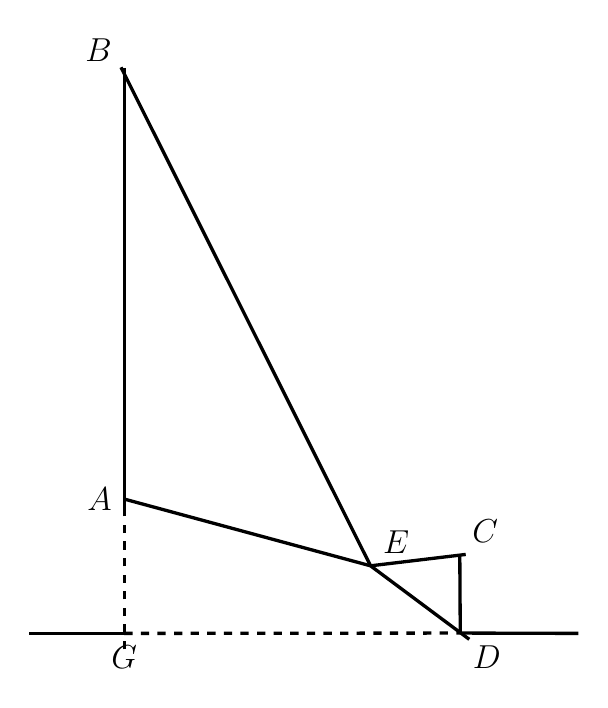
\begin{tikzpicture}[x=0.015066cm, y=0.015066cm, line join=round, line width=1.2pt]

% Named points (pixel x, 604 - pixel y)
\coordinate (B) at (104,538);
\coordinate (A) at (104,179.3);
\coordinate (G) at (104,66);
\coordinate (C) at (387,132);
\coordinate (D) at (387.4,66.3);
\coordinate (E) at (311.75,123);

% Dashed construction line (vertical x=104 px)
\draw[dashed] (104,52.6) -- (104,244.4);

% Baseline y=538 px: solid outer extensions, dashed G-D stretch
\draw (24,66) -- (G);                       % solid left extension
\draw[dashed] (G) -- (D);                   % dashed G-D stretch
\draw (D) -- (487,66);                      % solid right extension

% Solid segments, all terminating exactly at E
\draw (101.3,543.4) -- (E);                 % B to E
\draw (104,543) -- (104,166);               % vertical through B and A
\draw (A) -- (E);                           % A to E (trimmed at E)
\draw (C) -- (D);                           % C-D vertical, plain ends at C and D
\draw (395,61) -- (E);                      % branch from (395,543)px to E (trimmed at E)
\draw (392,132.6) -- (E);                   % second branch to E (trimmed at E)

% Labels
\fontsize{12}{14.4}\selectfont
\node[above left] at (B) {$B$};
\node[left] at (A) {$A$};
\node[above right] at (C) {$C$};
\node[above right] at (E) {$E$};
\node[below] at (G) {$G$};
\node[below right] at (D) {$D$};

\end{tikzpicture}
\end{document}